% Options for packages loaded elsewhere
\PassOptionsToPackage{unicode}{hyperref}
\PassOptionsToPackage{hyphens}{url}
%
\documentclass[
  man]{apa7}
\usepackage{amsmath,amssymb}
\usepackage{lmodern}
\usepackage{iftex}
\ifPDFTeX
  \usepackage[T1]{fontenc}
  \usepackage[utf8]{inputenc}
  \usepackage{textcomp} % provide euro and other symbols
\else % if luatex or xetex
  \usepackage{unicode-math}
  \defaultfontfeatures{Scale=MatchLowercase}
  \defaultfontfeatures[\rmfamily]{Ligatures=TeX,Scale=1}
\fi
% Use upquote if available, for straight quotes in verbatim environments
\IfFileExists{upquote.sty}{\usepackage{upquote}}{}
\IfFileExists{microtype.sty}{% use microtype if available
  \usepackage[]{microtype}
  \UseMicrotypeSet[protrusion]{basicmath} % disable protrusion for tt fonts
}{}
\makeatletter
\@ifundefined{KOMAClassName}{% if non-KOMA class
  \IfFileExists{parskip.sty}{%
    \usepackage{parskip}
  }{% else
    \setlength{\parindent}{0pt}
    \setlength{\parskip}{6pt plus 2pt minus 1pt}}
}{% if KOMA class
  \KOMAoptions{parskip=half}}
\makeatother
\usepackage{xcolor}
\usepackage{graphicx}
\makeatletter
\def\maxwidth{\ifdim\Gin@nat@width>\linewidth\linewidth\else\Gin@nat@width\fi}
\def\maxheight{\ifdim\Gin@nat@height>\textheight\textheight\else\Gin@nat@height\fi}
\makeatother
% Scale images if necessary, so that they will not overflow the page
% margins by default, and it is still possible to overwrite the defaults
% using explicit options in \includegraphics[width, height, ...]{}
\setkeys{Gin}{width=\maxwidth,height=\maxheight,keepaspectratio}
% Set default figure placement to htbp
\makeatletter
\def\fps@figure{htbp}
\makeatother
\setlength{\emergencystretch}{3em} % prevent overfull lines
\providecommand{\tightlist}{%
  \setlength{\itemsep}{0pt}\setlength{\parskip}{0pt}}
\setcounter{secnumdepth}{-\maxdimen} % remove section numbering
% Make \paragraph and \subparagraph free-standing
\ifx\paragraph\undefined\else
  \let\oldparagraph\paragraph
  \renewcommand{\paragraph}[1]{\oldparagraph{#1}\mbox{}}
\fi
\ifx\subparagraph\undefined\else
  \let\oldsubparagraph\subparagraph
  \renewcommand{\subparagraph}[1]{\oldsubparagraph{#1}\mbox{}}
\fi
\newlength{\cslhangindent}
\setlength{\cslhangindent}{1.5em}
\newlength{\csllabelwidth}
\setlength{\csllabelwidth}{3em}
\newlength{\cslentryspacingunit} % times entry-spacing
\setlength{\cslentryspacingunit}{\parskip}
\newenvironment{CSLReferences}[2] % #1 hanging-ident, #2 entry spacing
 {% don't indent paragraphs
  \setlength{\parindent}{0pt}
  % turn on hanging indent if param 1 is 1
  \ifodd #1
  \let\oldpar\par
  \def\par{\hangindent=\cslhangindent\oldpar}
  \fi
  % set entry spacing
  \setlength{\parskip}{#2\cslentryspacingunit}
 }%
 {}
\usepackage{calc}
\newcommand{\CSLBlock}[1]{#1\hfill\break}
\newcommand{\CSLLeftMargin}[1]{\parbox[t]{\csllabelwidth}{#1}}
\newcommand{\CSLRightInline}[1]{\parbox[t]{\linewidth - \csllabelwidth}{#1}\break}
\newcommand{\CSLIndent}[1]{\hspace{\cslhangindent}#1}
\ifLuaTeX
\usepackage[bidi=basic]{babel}
\else
\usepackage[bidi=default]{babel}
\fi
\babelprovide[main,import]{english}
% get rid of language-specific shorthands (see #6817):
\let\LanguageShortHands\languageshorthands
\def\languageshorthands#1{}
% Manuscript styling
\usepackage{upgreek}
\captionsetup{font=singlespacing,justification=justified}

% Table formatting
\usepackage{longtable}
\usepackage{lscape}
% \usepackage[counterclockwise]{rotating}   % Landscape page setup for large tables
\usepackage{multirow}		% Table styling
\usepackage{tabularx}		% Control Column width
\usepackage[flushleft]{threeparttable}	% Allows for three part tables with a specified notes section
\usepackage{threeparttablex}            % Lets threeparttable work with longtable

% Create new environments so endfloat can handle them
% \newenvironment{ltable}
%   {\begin{landscape}\centering\begin{threeparttable}}
%   {\end{threeparttable}\end{landscape}}
\newenvironment{lltable}{\begin{landscape}\centering\begin{ThreePartTable}}{\end{ThreePartTable}\end{landscape}}

% Enables adjusting longtable caption width to table width
% Solution found at http://golatex.de/longtable-mit-caption-so-breit-wie-die-tabelle-t15767.html
\makeatletter
\newcommand\LastLTentrywidth{1em}
\newlength\longtablewidth
\setlength{\longtablewidth}{1in}
\newcommand{\getlongtablewidth}{\begingroup \ifcsname LT@\roman{LT@tables}\endcsname \global\longtablewidth=0pt \renewcommand{\LT@entry}[2]{\global\advance\longtablewidth by ##2\relax\gdef\LastLTentrywidth{##2}}\@nameuse{LT@\roman{LT@tables}} \fi \endgroup}

% \setlength{\parindent}{0.5in}
% \setlength{\parskip}{0pt plus 0pt minus 0pt}

% Overwrite redefinition of paragraph and subparagraph by the default LaTeX template
% See https://github.com/crsh/papaja/issues/292
\makeatletter
\renewcommand{\paragraph}{\@startsection{paragraph}{4}{\parindent}%
  {0\baselineskip \@plus 0.2ex \@minus 0.2ex}%
  {-1em}%
  {\normalfont\normalsize\bfseries\itshape\typesectitle}}

\renewcommand{\subparagraph}[1]{\@startsection{subparagraph}{5}{1em}%
  {0\baselineskip \@plus 0.2ex \@minus 0.2ex}%
  {-\z@\relax}%
  {\normalfont\normalsize\itshape\hspace{\parindent}{#1}\textit{\addperi}}{\relax}}
\makeatother

% \usepackage{etoolbox}
\makeatletter
\patchcmd{\HyOrg@maketitle}
  {\section{\normalfont\normalsize\abstractname}}
  {\section*{\normalfont\normalsize\abstractname}}
  {}{\typeout{Failed to patch abstract.}}
\patchcmd{\HyOrg@maketitle}
  {\section{\protect\normalfont{\@title}}}
  {\section*{\protect\normalfont{\@title}}}
  {}{\typeout{Failed to patch title.}}
\makeatother

\usepackage{xpatch}
\makeatletter
\xapptocmd\appendix
  {\xapptocmd\section
    {\addcontentsline{toc}{section}{\appendixname\ifoneappendix\else~\theappendix\fi\\: #1}}
    {}{\InnerPatchFailed}%
  }
{}{\PatchFailed}
\keywords{Gender diversity, Gender categorization, Transgender, Measurement\newline\indent Word count: 3557}
\DeclareDelayedFloatFlavor{ThreePartTable}{table}
\DeclareDelayedFloatFlavor{lltable}{table}
\DeclareDelayedFloatFlavor*{longtable}{table}
\makeatletter
\renewcommand{\efloat@iwrite}[1]{\immediate\expandafter\protected@write\csname efloat@post#1\endcsname{}}
\makeatother
\usepackage{csquotes}
\makeatletter
\renewcommand{\paragraph}{\@startsection{paragraph}{4}{\parindent}%
  {0\baselineskip \@plus 0.2ex \@minus 0.2ex}%
  {-1em}%
  {\normalfont\normalsize\bfseries\typesectitle}}

\renewcommand{\subparagraph}[1]{\@startsection{subparagraph}{5}{1em}%
  {0\baselineskip \@plus 0.2ex \@minus 0.2ex}%
  {-\z@\relax}%
  {\normalfont\normalsize\bfseries\itshape\hspace{\parindent}{#1}\textit{\addperi}}{\relax}}
\makeatother

\ifLuaTeX
  \usepackage{selnolig}  % disable illegal ligatures
\fi
\IfFileExists{bookmark.sty}{\usepackage{bookmark}}{\usepackage{hyperref}}
\IfFileExists{xurl.sty}{\usepackage{xurl}}{} % add URL line breaks if available
\urlstyle{same} % disable monospaced font for URLs
\hypersetup{
  pdftitle={The effect of response options on gender categorization ( provisional title)},
  pdfauthor={Elli van Berlekom1 \& Coauthors1,2},
  pdflang={en-EN},
  pdfkeywords={Gender diversity, Gender categorization, Transgender, Measurement},
  hidelinks,
  pdfcreator={LaTeX via pandoc}}

\title{The effect of response options on gender categorization ( provisional title)}
\author{Elli van Berlekom\textsuperscript{1} \& Coauthors\textsuperscript{1,2}}
\date{}


\shorttitle{Rsponse options and gender categorization}

\authornote{

Add complete departmental affiliations for each author here. Each new line herein must be indented, like this line.

Data \& scripts are available at osf link. The authors declare no conflict of interest.

The authors made the following contributions. Elli van Berlekom: Conceptualization, Writing - Original Draft Preparation, Writing - Review \& Editing; Coauthors: A lot of things, Author order TBD.

Correspondence concerning this article should be addressed to Elli van Berlekom, Albanovägen 12. E-mail: \href{mailto:elli.vanberlekom@psychology.su.se}{\nolinkurl{elli.vanberlekom@psychology.su.se}}

}

\affiliation{\vspace{0.5cm}\textsuperscript{1} Stockholm University\\\textsuperscript{2} Lund University}

\abstract{%
Gender categorizations studies almost exclusively measure outcomes in terms of woman and men only. However, this does not capture the diversity of gender and may produce inaccurate results. Consequently, this study investigated the effect of response options on binary gender categorization (N = 120). The findings suggest that participants are more likely to categorize gender beyond the binary when provided with explicit response options, such as ``non-binary'' and ``I don't know''. The results are consistent with previous research on the importance of including flexible response options to better express oneself. However, it was also found that increased freedom did not necessarily increase gender diversity in participants' categorizations. The study highlights the importance of careful consideration of response options in gender categorization research. Future research may benefit from utilizing a variety of response options, including open text-boxes, forced choice-alternatives, and dimensional scales.
}



\begin{document}
\maketitle

Precision is key when measuring constructs in psychological research. One domain where precision is lacking is in the use of binary response options for gender (i.e.~``woman'' and ``man''), which fails to capture the complex and fluid nature of gender/sex (Hyde et al., 2018; Lindqvist et al., 2020). While researchers have begun offering participants more flexible options to define their gender (Lindqvist et al., 2020; Saperstein \& Westbrook, 2021), such as additional categories or free text responses, studies still predominantly use binary gender options when categorizing participants. Thus, understanding of how participants' response measures affect gender categorization remains limited Therefore, the current study aims to test how non-binary alternatives affect gender categorization.

Bem (n.d.) was a pioneer in challenging the dichotomous and binary conceptualizations of gender. Bem developed the first scale (the Bem Sex Role inventory, BSRI, 1974) to measure femininity and masculinity as separate traits, finding that many individuals exhibit a mixture of feminine and masculine traits. The BSRI has been used more often as self-reports of gender as a trait. More recently, several guides have been developed that recommend the use of open free text options or multiple options (e.g., woman, man, other, nonbinary). when asking participants to indicate their gender (see for example Lindqvist et al., 2020). When participants have given such options, they use them to indicate a gender identity other than women or men. Although this practice is still far from the norm, it is becoming increasingly commonplace for researchers to measure gender of participants in this open-ended way (Carleton et al., 2022; Cronin et al., 2022; D'Agostino et al., 2022; Göttgens et al., 2022)

In contrast, the literature on gender categorization of others still almost exclusively treats gender as a binary category. Gender categorization is a cognitive process that occurs when individuals perceive others (Kang \& Bodenhausen, 2015). Researchers in this field have explored the speed and automaticity of gender perception in faces, as well as which facial features are associated with specific gender categories, such as women and men (e.g. Mogilski \& Welling, 2018) . Generally, the findings indicate that gender is rapidly and automatically categorized (Habibi \& Khurana, 2012; Jung et al., 2019), with facial features such as skin smoothness, jawline, and hair length used to determine gender identity. Lastly, studies in this field have indicated that people perceive faces categorically (Campanella et al., 2001). In other words, that faces, even when manipulated to vary on a continuum from feminine to masculine were still perceived as belonging to the categories women or man. However, these studies typically do reflect the diverse nature of gender or consider alternative response options (ref).

Instead, gender categorization is most often measured through a forced-choice task in which participants are forced to indicate either ``female'' or ``male'' when presented with a face (see for example Campanella et al., 2001; Cloutier et al., 2005; Webster et al., 2004; Zhao \& Bentin, 2008). A slightly different approach asks participants to rate faces on a gender gradation as a quality, often using ``feminine'' and ``masculine'' as endpoints on a single gradation (D'Ascenzo et al., 2014). Only in some rare cases are masculinity and femininity measued using different gradations for femininity and masculinity (e.g. Wittlin et al., 2018). Despite some variations therefore, the literature overwhelmingly presents gender as a binary in studies of gender categorization of others.

The use of binary gender measures presents significant problems in accurately reflecting the diversity of gender. Such measures reinforce the notion of gender as a binary concept, thereby invalidating non-binary genders. This not only misrepresents the reality of gender but also perpetuates discriminatory attitudes towards non-binary individuals. Consequently, it is imperative to test alternative measures that acknowledge and respect the diversity of gender identities.

\hypertarget{overview-of-the-present-research}{%
\subsection{Overview of the present research}\label{overview-of-the-present-research}}

Across two experiments, we investigate how alternative response options impact gender categorization. The purpose of both experiment was to answer the following three research questions
\emph{Research question 1}: Do participants categorize gender beyond the binary when response options allow them to do so?
\emph{Research question 2}: Two what extent do beyond-binary responses affect the distribution of woman/man responses?
\emph{Research question 3}: Can response options which do not present the categories of woman and man as oppositional reduce categorical perception.

Research questions 1 and 2 were investigated in study 1 and research question 3 was investigated in study 2.

\hypertarget{study-1}{%
\section{Study 1}\label{study-1}}

Study 1 tested whether response options that allow categorization beyond the binary influences people to categorize gender beyond the binary. Accordingly, Experiment 1 manipulated response options.The specific alternatives were based on common practices for self-identification of gender. To avoid suggesting that gender only consists of women and men, these studies recommend including a third option. Moreover, given that gender may not always be evident from a person's countenance, an ``I don't know'' option should also be incorporated into the task. This suggests that a forced choice task is best supplemented with both an ``other'' option and an ``I don't know'' option. Another common practice is to give people an open text box in which they may type in whatever they like. This method has been recommended by different researchers (Lindqvist et al., 2020; Saperstein \& Westbrook, 2021). This method has the benefit of affording participants freedom to answer as they choose.Therefore the study included three conditions (Binary categories, Multiple categories and Free text options).

\hypertarget{method}{%
\section{Method}\label{method}}

\hypertarget{participants}{%
\subsection{Participants}\label{participants}}

Swedish participants (\emph{N} = 68) were recruited through advertising online and on the university campus (\emph{M}\textsubscript{age}= 37.67, \emph{SD}\textsubscript{age} = 14.56, Range = 20 - 69). Self-identified gender was measured using an open-ended text box; participants were 35 women, 32 men and 1 who did not indicate gender). All participants were informed that participation was voluntary, that they could withdraw from the study and that results do no include any identifying features. In accordance with ethical guidelines, all participants provided written informed consent.

\hypertarget{stimuli}{%
\subsection{Stimuli}\label{stimuli}}

Faces used for the gender categorization task were produced using the London Face Database (deBruine) and the Chicago Face Database (ref) morphed with on Webmorph (ref). For Black, Asian and White faces, the six most feminine faces of women and the six most masculine faces of men were selected, using the codebook provided by the researchers. The faces were matched, so that the most feminine faces in the database were morphed with the most masculine faces. The morphs were made in 7 steps, from completely feminine to completely masculine. Because there were 18 pairs morphed in 7 steps, the total number of faces was 126. Each pair of faces were morphed in 7 steps, from completely feminine to completely masculine resulting in a total number of 126 faces (see Figure~\ref{fig:insert}, which should include percentage femininity of the face )

\hypertarget{measures}{%
\subsection{Measures}\label{measures}}

The primary outcome was responses to the categorization task. For analysis purposes, these were aggregated in the following ways:

\emph{Beyond-binary categorizations} represented the categories where participants did not categorise the face as woman or man. This was a dichotomous variable that was calculated from the categorization data by combining the responses of ``I don't know'' and ``non-binary''. These beyond-binary responses were coded as 1 and binary responses as 0.

\emph{Binary categorization} represented only the responses that were either woman (coded as 1) or man (coded as 0). All other responses were removed from this dataset.

\hypertarget{procedure}{%
\subsection{Procedure}\label{procedure}}

Participants completed the experiment on a computer in a quiet room. Each trial consisted of a face accompanied by the question ``How would you gender categorize this person?''. Each person completed a total of 126 trials (i.e.~they categorized every face in the stimuli set). Participants were randomly allocated into one of the three response options conditions: binary categories, multiple categories, and free text. In the binary categories condition, the only option to respond was ``woman'' and ``man''. he multiple categories conditionincluded the options ``other'' and ``I don't know'' as well as woman or man. the free text condition consisted of an open text box.

\hypertarget{data-analysis}{%
\subsection{Data analysis}\label{data-analysis}}

We used R (Version 4.2.2; R Core Team, 2022) and the R-packages \emph{papaja} (Version 0.1.1; Aust \& Barth, 2022), \emph{shiny} (Version 1.7.4; Chang et al., 2022), and \emph{tinylabels} (Version 0.2.3; Barth, 2022). Descriptive statistics were used to summarize the data, and Bayesian mixed-effects models were used to test the research questions. For all models, we included varying intercepts for both participants and trials. To answer each research question, we used a two-step approach which began with a model comparison approach followed by Bayes factor tests of specific contrasts. In all cases, the models included varying intercepts for both participants trials.

\hypertarget{research-question-1-the-use-of-categories-beyond-the-binary}{%
\subsubsection{Research question 1: The use of categories beyond the binary}\label{research-question-1-the-use-of-categories-beyond-the-binary}}

In research question one, we investigated whether participants categorized faces beyond the binary when given the chance. This could manifest as either a main effect of condition or an interaction between condition and morph level if categorizations beyond the binary were limited to only the most androgynous faces. For this analyses, the Binary categories condition was excluded, as that condition precluded the possibility of categorizing beyond the binary. The specific questions then, were ``do people categorize faces beyond the binary?'', ``does this effect depend on condition?'' and ``are ambiguous faces more likely to be categorized beyond the binary?''. These questions correspond to main effects of response option condition, facial morph level and an interaction between the two.

Accordingly, the models were fit to the outcome \emph{Beyond-binary categorizations} and comprised a Null model with no additional predictors, a Main effects model and an Interaction model For full model specification (including priors) and model diagnostics, see the supplementary material. These model were then compared in terms of predictive power on out-of-sample data points, estimated using Leave-one-out cross validation (LOO-CV). This represents an indirect test of the research questions, and can be viewed as an imperfect analogy to checking whether there is a ``significant'' overall interaction in a classical F-test.

As a more direct test, we also calculated the Bayes Factor for the specific contrasts suggested by these questions. In other words, we compared the overall probability of making categorizations beyond the binary in the Free text condition and the Multiple categories conditions. Additionally,
we compared the prevalence of categorization beyond the binary specifically of the most androgynous faces. The Bayes factors were compared the null hypothesis that the contrast was equal to 0 and calculated using the Savage-Dickey Density Ratio.

\hypertarget{research-question-2-the-distribution-of-binary-responses}{%
\subsubsection{Research question 2: The distribution of binary responses}\label{research-question-2-the-distribution-of-binary-responses}}

In research question two, we investigated whether the distribution of \emph{binary responses} was different depending on response option condition. This could manifest as a main effect of condition if there was an overall skew in the results or as an interaction between condition and morph level, in case that the skew was isolated to just one level of morph (for example at the middle).

Similar to RQ1, this data was tested using with Bayesian mixed models fitted to the data. This included an initial model comparison approach, with Null model, and Main Effects model and an Interaction Model. If the model comparison did not preclude the Interaction model, we tested the contrast of the overall distribution as well as isolated to whichever morph level, a visual inspection of the data suggested was the most strongly skewed.

\hypertarget{results}{%
\section{Results}\label{results}}

The raw distribution of gender categorizations made by participants is presented in Figure~\ref{fig:descriptives}.

\emph{to do: fix the bug that is producing those ugly red lines at the bottom of this figure}

\begin{figure}
\centering
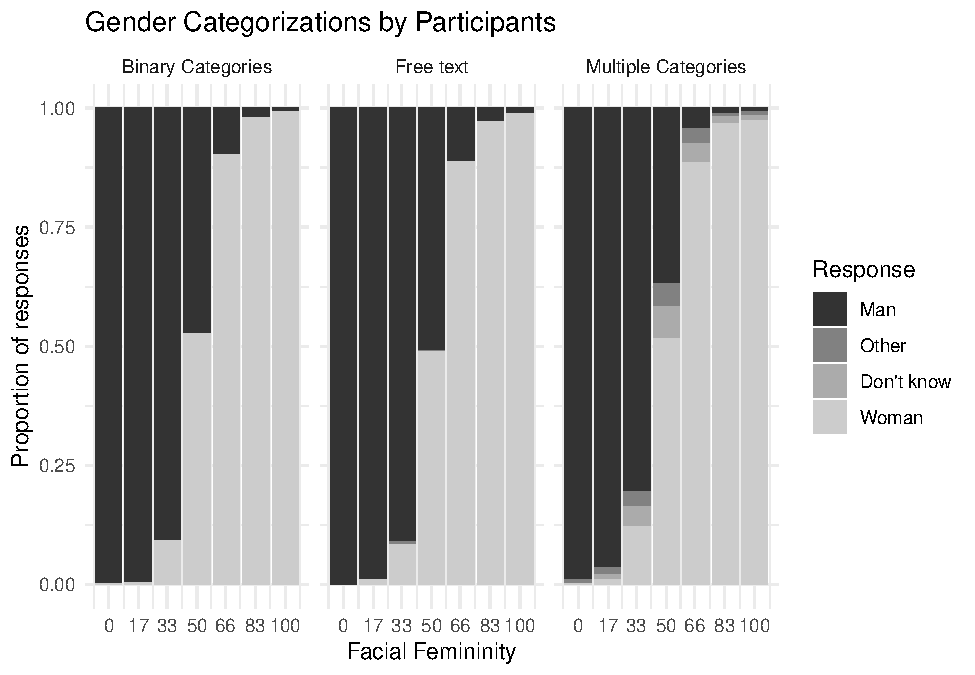
\includegraphics{resp_opts_manus23022_files/figure-latex/descriptives-1.pdf}
\caption{\label{fig:descriptives}Gender Categorizations by Participants}
\end{figure}

To investigate whether response options affected gender categorization we fit a Null Model, a Main Effects Model and an interaction model to the data. As stated, for these analyses, the Binary Categories condition was excluded, as participant did not have the option to categorize beyond the binary. The results of model comparison are presented in Table~\ref{tab:loo}.
Table~\ref{tab:loo} suggests that the Interaction model is the most predictive. However the absolute difference between the Interaction model and the Main effects model is small and importantly, the difference is small in relation to the standard error of the difference. This suggests that the data is inconclusive about which model is most suitable, although both are superior to the Null model. As model comparison did not conclusively preclude the Interaction model, we continued by testing specific, relevant contrasts using the Interaction model (see the Supplementary material for specific contrast weights).

\begin{table}

\caption{\label{tab:loo}Relative predictive power of models describing the outcome on the categorization task}
\centering
\begin{threeparttable}
\begin{tabular}[t]{lcccc}
\toprule
  & LOO diff & St. Error diff & LOO & St. Error LOO\\
\midrule
Interaction & 0.00 & 0.00 & -234.17 & 23.23\\
Main Effect & -2.46 & 2.71 & -236.63 & 23.07\\
Null & -18.83 & 6.02 & -253.00 & 24.51\\
\bottomrule
\end{tabular}
\begin{tablenotes}[para]
\item \textit{Note.} 
\item LOO diff refers to the difference in loo between the model and the most predictive model. The first row describes the most predictive model, which is why the difference is 0
\end{tablenotes}
\end{threeparttable}
\end{table}

\begin{figure}
\centering
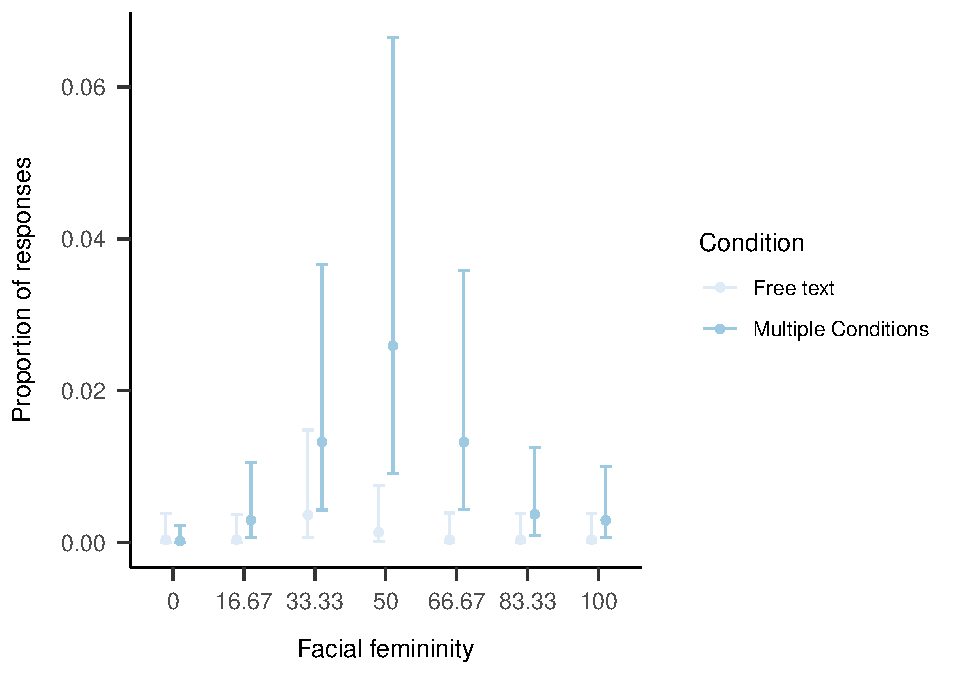
\includegraphics{resp_opts_manus23022_files/figure-latex/exp-one-inf-1.pdf}
\caption{\label{fig:exp-one-inf}Proportion of beyond-binary responses in the Multiple Categories and Free Text conditions}
\end{figure}

Model parameters are visualized in Figure~\ref{fig:exp-one-inf}. First, whether participants overall made more beyond-binary categorizations in the multiple categories condition than in the free text condition. Although the incidence was rare in both conditions () The evidence suggests fairly convincingly that this is the case (OR = 0.02, CI ={[}0.00, 0.21{]}, BF\textsubscript{10}= 97.67). Additionally, based on visual inspection of Figure~\ref{fig:exp-one-inf}, which suggested that the difference between the condition was concentrated at morphs containing equal levels of femininity and masculinity (i.e.~morph level 50) we explored whether the evidence supported this difference at morph level 50. The evidence was in favor of this difference (OR = 0.02, CI ={[}0.00, 0.26{]}, BF\textsubscript{10}= 17). Lastly, we tested the difference using quadratic weights, though here the difference was inconclusive (OR = 0.82, CI = {[}0.44,1.58{]}, BF\textsubscript{10}= 0.53).

Overall the evidence suggests at least somewhat strongly that when participants have the option of using beyond-binary response options, they use them.

Subsequently, we tested whether the inclusion of non-binary response options skewed the distribution of categorization of faces as women and men. For this analysis, therefore, we tested the outcome variable \emph{binary categorization}, excluding ``other'' ``I don't know'' and any other respones in the free text.

\begin{table}

\caption{\label{tab:rq2-table}Relative predictive power of models describing the outcome on the categorization task}
\centering
\begin{threeparttable}
\begin{tabular}[t]{llccc}
\toprule
  & LOO difference & St. Error diff & LOO & St. Error LOO\\
\midrule
morph\_only & 0.00 & 0.00 & -1343.71 & 43.17\\
main\_effects & -1.85 & 0.86 & -1345.56 & 43.17\\
condition\_only & -4.98 & 5.26 & -1348.69 & 44.49\\
Null & -5.36 & 4.88 & -1349.07 & 44.12\\
interaction & -6.69 & 3.02 & -1350.40 & 43.48\\
\bottomrule
\end{tabular}
\begin{tablenotes}[para]
\item \textit{Note.} 
\item LOO diff refers to the difference in loo between the model and the most predictive model. The first row describes the most predictive model, which is why the difference is 0
\end{tablenotes}
\end{threeparttable}
\end{table}

To test this research question, we first carried out model comparison. The results of this are presented in Table~\ref{tab:rq2-table}. Again, we compared a Null model, a Main Effects model and an Interaction model. Although the Interaction model was the worst in terms of LOO-CV, the standard errors were quite large relative to the difference, again suggesting that the model comparison was inconclusive and the existance of an interaction could not be excluded. For completeness we therefore carried out the contrast analyses using the Interaction model.

Based on the pattern in Figure~\ref{fig:descriptives}, which seems to show that in the Multiple Categories condition, participants made fewer Man responses compared to the other condition, we compared the distribution of woman/man responses at morph level 50. The evidence were slightly in favor of there being no difference between the multiple categories and the free text conditions (OR = 0.61, CI ={[}0.29, 1.28{]}, BF\textsubscript{01}= 4.79) and moderately in favor of no difference between multiple categories and binary categories conditions (OR = 0.76, CI ={[}0.37, 1.57{]}, BF\textsubscript{01}= 9.08). In other words, the evidence suggests that when participants categories faces beyond the binary, this does not skew the categorizations of women and men in any direction.

\hypertarget{discussion}{%
\section{Discussion}\label{discussion}}

Eexperiment 1 indicated that participants categorize beyond the binary when response options include more options than women and men only. However, the free text option did not differ from the binary option. Thus, the written out choices seem to act as reminders to participants. Furthermore, categorization beyond the binary affected former man and women responses to similar degrees, meaning that the ratio of women and men were still about 50/50. This did not systematically affect their overall pattern of responses in terms of woman and man categorizations.

\hypertarget{study-2}{%
\section{Study 2}\label{study-2}}

Study 2 tested whether continuous scales that measure woman and men separately reduce categorical perception. To that end, we once again borrowed from the literature on self-categorization, this time using Bem's (1978) method of measuring gender on two separate scales.
If categorical perception occurs, ratings of woman and man should be skewed near the 50/50 morph level. In other words, a face with 33.33\% woman would be rated as less woman than that. Therefore, we examined the differences between the two conditions at morph levels 33.33\% and 66.67\% morph.

\hypertarget{method-1}{%
\section{Method}\label{method-1}}

\hypertarget{participants-1}{%
\subsubsection{Participants}\label{participants-1}}

Participants (\emph{N} = 49) were recruited through advertising online and on the university campus (\emph{M}\textsubscript{age}= 36.67, \emph{SD}\textsubscript{age} = 12.54).Self-identified gender was measured using an open-ended text box; 25 women and 24 men participated. Participants were monetarily compensated for their time. All participants were informed that participation was voluntary and gave written consent to participate in the study in accordance with ethical recommendations. The participants were randomly allocated to conditions.

\hypertarget{stimuli-procedure}{%
\subsection{Stimuli \& Procedure}\label{stimuli-procedure}}

The stimuli and procedure for study 2 were identical to experiment 1 but included only two conditions. Study 2 differed only the response options conditions, such that esponse option conditions consisted of a single dimension, which ranged from ``woman'' to ``man'' and ``multiple dimension'' which ranged from ``not woman'' to ``woman'' and ``not man'' to ``man''. For the multiple dimensions condition, participants rated the same faces according to both scales, but on separate trials. Although Bem (1978) used scales of femininity and masculinity, the anchors were chosen because gender categorization was the focus of the present study.

\hypertarget{data-analysis-1}{%
\subsection{Data analysis}\label{data-analysis-1}}

Research question 3 asked whether whether participants would view faces less categorically in when they categorized them using multiple dimensions (i.e.~Not woman - Woman/Not man -Man) than when they used the single dimension (Woman-Man). We expected to see a difference between the two conditions at morph levels 33.33 and 66.67 as these were the closes to the midwaty point. In other words, if categorical perception is reduced, we would expect to see an interaction between condition and morph level, but not a main effect. To test this, we fit a single Bayesian mixed-effects model which calculated unique fixed intercepts at each intersection of morph level and condition as well as varying intercepts for participants and faces (See supplemental material for full model specification). Using Savage-Dickey density ratios, we calculated the Bayes Factors for the contrasts between single dimension condition and multiple dimension at morph level 33.37 and 66.66 only.

\hypertarget{results-1}{%
\section{Results}\label{results-1}}

The mean ratings in both conditions are presented in Figure~\ref{fig:descriptives-two}.

\begin{figure}
\centering
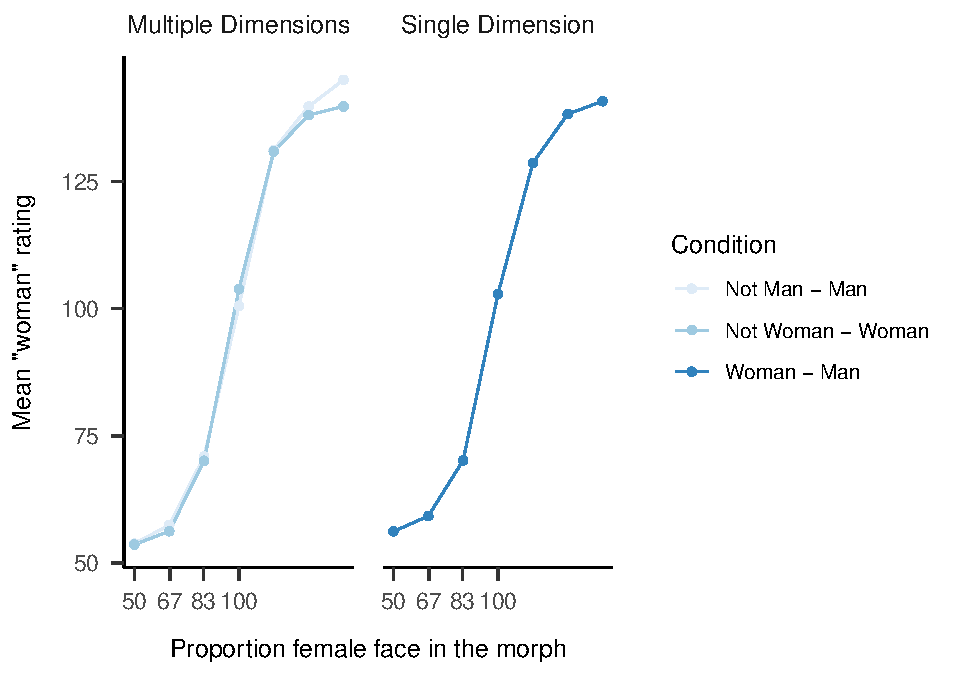
\includegraphics{resp_opts_manus23022_files/figure-latex/descriptives-two-1.pdf}
\caption{\label{fig:descriptives-two}Mean ratings of faces in Single dimension and multiple dimensions}
\end{figure}

\begin{figure}
\centering
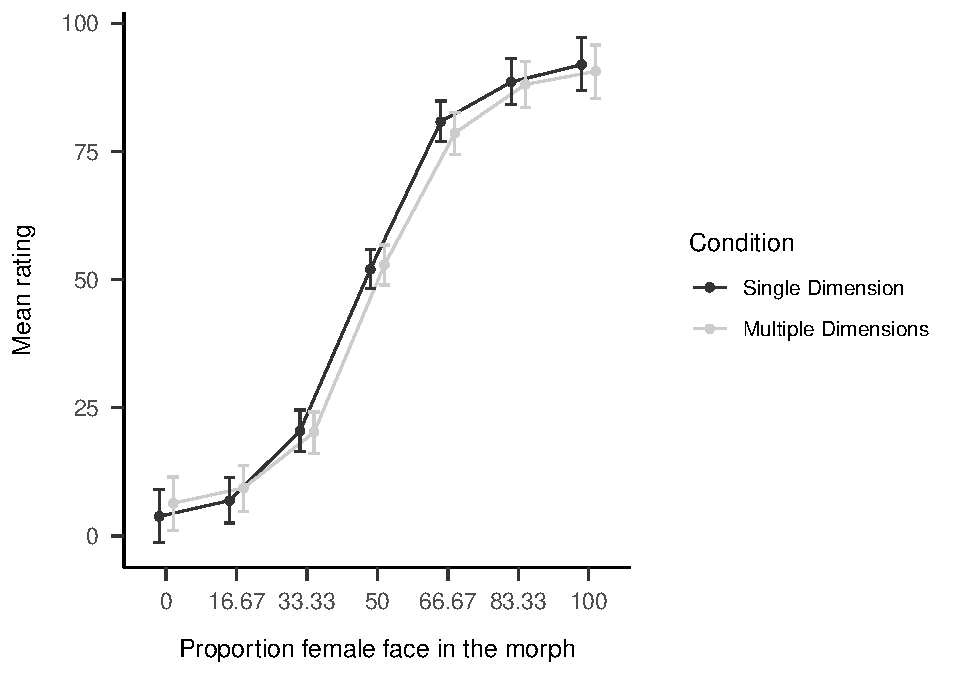
\includegraphics{resp_opts_manus23022_files/figure-latex/exp-two-inf-1.pdf}
\caption{\label{fig:exp-two-inf}Mean gender ratings in Single Dimension and Multiple Dimensions conditions}
\end{figure}

We compared the mean rating at 33.33 morph and at 66.67 morph for both conditions. At 33.33 the evidence strongly suggested that the two conditions were the same
(Estimate = 0.28, CI ={[}-3.91, 4.51{]}, BF\textsubscript{01}= 31.57). This was also the case at 66.67
(Estimate = 2.29, CI ={[}-2.03, 6.57{]}, BF\textsubscript{01}= 19.17). Overall, both conditions showed fairly strong tendencies toward categorical perception and they did not differ in this regard.

\hypertarget{discussion-1}{%
\section{Discussion}\label{discussion-1}}

Experiment 2 showed that r response scales which did not present women and men as opposing categories did not changed participants categorical perception. Indeed a highly binary view of gender was present and participants treated womanhood and manhood as opposites although the scale would allow them to be more flexible.

\hypertarget{general-discussion}{%
\section{General discussion}\label{general-discussion}}

In two experiments, we tested how response options in gender categorization of others influence binary gender categorization. Specifically, the results provided strong evidence that participants only use beyond-binary options to categorize faces when such options are provided explicitly. Free text answers or continuous scales did not affect participants binary gender categorization.

These findings are somewhat consistent with previous research, such as the work of Saperstein and Westbrook (2018) and Lindqvist (2019), which has shown that including flexible response options allow participants to better express themselves. Unlike the literature on self-categorization, increased freedom did not increase the gender diversity of participants' categorizations, rather explicit reminders seem to have the largest effect. When participants categorized women or men on continuous scales, the results differ from Bem's (1978) who found that participants categorize their own femininity and masculinity independently of each other. Rather, when categorizing others, the participants in the present study seemed to treat women and men as opposites, even when the response options did not pose them as such.

It is worth noting that this study only examined participants' stated categorizations, and it is possible that they may have made other categorizations internally that were not reflected in their responses. However, it is important to recognize that a purely behavioral study such as this cannot fully capture the neurological processes underlying gender perception, which may require more sophisticated techniques such as fMRI and EEEG (Freeman et al 2010, Kloth et al, 2011).

In this study we aggregated responses that did not indicate woman or man. In the multiple response option condition, both ``I don't know'' and ``Non-binary'' were included as a beyond binary categorization. We justified this on the basis that what we are interested in is any categorization beyond the binary. However, these two options are not the same. Furthermore, it is important to note that no matter how a person looks like it is impossible to know their binary or non-binary gender identity (ref). Therefore, if a person aims to be inclusive and not categorize in a binary way, then ``I don't know'' options are better.

Based on these findings, we recommend researchers to carefully consider their measurements of gender categorization. Open text-boxes, forced choice-alternatives and dimensional scales are all viable alternatives. Even researchers who are primarily interested in binary categorizations should consider including beyond-binary alternatives, to avoid perpetuating cisgenderism and to accurately represent the diversity of gender.

\hypertarget{conclusion}{%
\paragraph{Conclusion}\label{conclusion}}

In two experiments we tested how different response alternatives affected gender categorizations. Participants were more likely to categorise faces beyond the binary when using a forced-choice paradigm including ``non-binary'' and ``I don't know'' than when using a free text option, or slider scales. In comparison to self-identification questions were open ended responses are preferred, other categorization might need response options that explicitly reminds participants that not all people identity as woman or man.

\newpage

\hypertarget{references}{%
\section{References}\label{references}}

\hypertarget{refs}{}
\begin{CSLReferences}{1}{0}
\leavevmode\vadjust pre{\hypertarget{ref-R-papaja}{}}%
Aust, F., \& Barth, M. (2022). \emph{{papaja}: {Prepare} reproducible {APA} journal articles with {R Markdown}}. \url{https://github.com/crsh/papaja}

\leavevmode\vadjust pre{\hypertarget{ref-R-tinylabels}{}}%
Barth, M. (2022). \emph{{tinylabels}: Lightweight variable labels}. \url{https://cran.r-project.org/package=tinylabels}

\leavevmode\vadjust pre{\hypertarget{ref-bem_measurement_nodate}{}}%
Bem, S. L. (n.d.). \emph{{THE} {MEASUREMENT} {OF} {PSYCHOLOGICAL} {ANDROGYNY}}. 8.

\leavevmode\vadjust pre{\hypertarget{ref-campanella_categorical_2001}{}}%
Campanella, S., Chrysochoos, A., \& Bruyer, R. (2001). Categorical perception of facial gender information: Behavioural evidence and the face-space metaphor. \emph{Visual Cognition}, \emph{8}(2), 237--262. \url{https://doi.org/10.1080/13506280042000072}

\leavevmode\vadjust pre{\hypertarget{ref-carleton_assessing_2022}{}}%
Carleton, R. N., McCarron, M., Krätzig, G. P., Sauer-Zavala, S., Neary, J. P., Lix, L. M., Fletcher, A. J., Camp, R. D., Shields, R. E., Jamshidi, L., Nisbet, J., Maguire, K. Q., MacPhee, R. S., Afifi, T. O., Jones, N. A., Martin, R. R., Sareen, J., Brunet, A., Beshai, S., \ldots{} Asmundson, G. J. G. (2022). Assessing the impact of the royal canadian mounted police ({RCMP}) protocol and emotional resilience skills training ({ERST}) among diverse public safety personnel. \emph{{BMC} Psychology}, \emph{10}(1), 295. \url{https://doi.org/10.1186/s40359-022-00989-0}

\leavevmode\vadjust pre{\hypertarget{ref-R-shiny}{}}%
Chang, W., Cheng, J., Allaire, J., Sievert, C., Schloerke, B., Xie, Y., Allen, J., McPherson, J., Dipert, A., \& Borges, B. (2022). \emph{Shiny: Web application framework for r}. \url{https://CRAN.R-project.org/package=shiny}

\leavevmode\vadjust pre{\hypertarget{ref-cloutier_perceptual_2005}{}}%
Cloutier, J., Mason, M. F., \& Macrae, C. N. (2005). The perceptual determinants of person construal: Reopening the social-cognitive toolbox. \emph{Journal of Personality and Social Psychology}, \emph{88}(6), 885--894. \url{https://doi.org/10.1037/0022-3514.88.6.885}

\leavevmode\vadjust pre{\hypertarget{ref-cronin_younger_2022}{}}%
Cronin, K. A., Leahy, M., Ross, S. R., Wilder Schook, M., Ferrie, G. M., \& Alba, A. C. (2022). Younger generations are more interested than older generations in having non-domesticated animals as pets. \emph{{PLOS} {ONE}}, \emph{17}(1), e0262208. \url{https://doi.org/10.1371/journal.pone.0262208}

\leavevmode\vadjust pre{\hypertarget{ref-dagostino_organizational_2022}{}}%
D'Agostino, M., Levine, H., Sabharwal, M., \& Johnson-Manning, A. C. (2022). Organizational practices and second-generation gender bias: A qualitative inquiry into the career progression of u.s. State-level managers. \emph{The American Review of Public Administration}, \emph{52}(5), 335--350. \url{https://doi.org/10.1177/02750740221086605}

\leavevmode\vadjust pre{\hypertarget{ref-dascenzo_imagining_2014}{}}%
D'Ascenzo, S., Tommasi, L., \& Laeng, B. (2014). Imagining sex and adapting to it: Different aftereffects after perceiving versus imagining faces. \emph{Vision Research}, \emph{96}, 45--52. \url{https://doi.org/10.1016/j.visres.2014.01.002}

\leavevmode\vadjust pre{\hypertarget{ref-gottgens_impact_2022}{}}%
Göttgens, I., Darweesh, S. K. L., Bloem, B. R., \& Oertelt-Prigione, S. (2022). The impact of multiple gender dimensions on health-related quality of life in persons with parkinson's disease: An exploratory study. \emph{Journal of Neurology}, \emph{269}(11), 5963--5972. \url{https://doi.org/10.1007/s00415-022-11228-2}

\leavevmode\vadjust pre{\hypertarget{ref-habibi_spontaneous_2012}{}}%
Habibi, R., \& Khurana, B. (2012). Spontaneous gender categorization in masking and priming studies: Key for distinguishing jane from john doe but not madonna from sinatra. \emph{{PLoS} {ONE}}, \emph{7}(2), e32377. \url{https://doi.org/10.1371/journal.pone.0032377}

\leavevmode\vadjust pre{\hypertarget{ref-hyde_future_2018}{}}%
Hyde, J. S., Bigler, R. S., Joel, D., Tate, C. C., \& Anders, S. M. van. (2018). The future of sex and gender in psychology: Five challenges to the gender binary. \emph{American Psychologist}. \url{https://doi.org/10.1037/amp0000307}

\leavevmode\vadjust pre{\hypertarget{ref-jung_automaticity_2019}{}}%
Jung, K. H., White, K. R. G., \& Powanda, S. J. (2019). Automaticity of gender categorization: A test of the efficiency feature. \emph{Social Cognition}, \emph{37}(2), 122--144. \url{https://doi.org/10.1521/soco.2019.37.2.122}

\leavevmode\vadjust pre{\hypertarget{ref-kang_multiple_2015}{}}%
Kang, S. K., \& Bodenhausen, G. V. (2015). Multiple identities in social perception and interaction: Challenges and opportunities. \emph{Annual Review of Psychology}, \emph{66}(1), 547--574. \url{https://doi.org/10.1146/annurev-psych-010814-015025}

\leavevmode\vadjust pre{\hypertarget{ref-lindqvist_what_2020}{}}%
Lindqvist, A., Sendén, M. G., \& Renström, E. A. (2020). What is gender, anyway: A review of the options for operationalising gender. \emph{Psychology \& Sexuality}, 1--13. \url{https://doi.org/10.1080/19419899.2020.1729844}

\leavevmode\vadjust pre{\hypertarget{ref-mogilski_relative_2018}{}}%
Mogilski, J. K., \& Welling, L. L. M. (2018). The relative contribution of jawbone and cheekbone prominence, eyebrow thickness, eye size, and face length to evaluations of facial masculinity and attractiveness: A conjoint data-driven approach. \emph{Frontiers in Psychology}, \emph{9}, 2428. \url{https://doi.org/10.3389/fpsyg.2018.02428}

\leavevmode\vadjust pre{\hypertarget{ref-R-base}{}}%
R Core Team. (2022). \emph{R: A language and environment for statistical computing}. R Foundation for Statistical Computing. \url{https://www.R-project.org/}

\leavevmode\vadjust pre{\hypertarget{ref-saperstein_categorical_2021}{}}%
Saperstein, A., \& Westbrook, L. (2021). Categorical and gradational: Alternative survey measures of sex and gender. \emph{European Journal of Politics and Gender}, \emph{4}(1), 11--30. \url{https://doi.org/10.1332/251510820X15995647280686}

\leavevmode\vadjust pre{\hypertarget{ref-webster_adaptation_2004}{}}%
Webster, M. A., Kaping, D., Mizokami, Y., \& Duhamel, P. (2004). Adaptation to natural facial categories. \emph{Nature}, \emph{428}(6982), 557--561. \url{https://doi.org/10.1038/nature02420}

\leavevmode\vadjust pre{\hypertarget{ref-wittlin_about_2018}{}}%
Wittlin, N. M., Dovidio, J. F., LaFrance, M., \& Burke, S. E. (2018). About face: Memory for transgender versus cisgender targets' facial appearance. \emph{Journal of Experimental Social Psychology}, \emph{78}, 77--92. \url{https://doi.org/10.1016/j.jesp.2018.04.009}

\leavevmode\vadjust pre{\hypertarget{ref-zhao_own-_2008}{}}%
Zhao, L., \& Bentin, S. (2008). Own- and other-race categorization of faces by race, gender, and age. \emph{Psychonomic Bulletin \& Review}, \emph{15}(6), 1093--1099. \url{https://doi.org/10.3758/PBR.15.6.1093}

\end{CSLReferences}


\end{document}
